\documentclass{article}
\usepackage[margin=1in]{geometry}
\usepackage{physics}
\usepackage{graphicx}
\usepackage{caption}
\usepackage{amsmath}
\usepackage{bm}
\usepackage{authblk}
\usepackage{empheq}
\usepackage{amsfonts}
\usepackage{esint}
\usepackage[makeroom]{cancel}
\usepackage{dsfont}
\usepackage{centernot}
\usepackage{mathtools}
\usepackage{bigints}
\usepackage{amsthm}
\theoremstyle{definition}
\newtheorem{defn}{Definition}[section]
\newtheorem{prop}{Proposition}[section]
\newtheorem{rmk}{Remark}[section]
\newtheorem{thm}{Theorem}[section]
\newtheorem{exmp}{Example}[section]
\newtheorem{prob}{Problem}[section]
\newtheorem{sln}{Solution}[section]
\newtheorem*{prob*}{Problem}
\newtheorem{exer}{Exercise}[section]
\newtheorem*{exer*}{Exercise}
\newtheorem*{sln*}{Solution}
\usepackage{empheq}
\usepackage{hyperref}
\usepackage{tensor}
\usepackage{xcolor}
\hypersetup{
	colorlinks,
	linkcolor={black!50!black},
	citecolor={blue!50!black},
	urlcolor={blue!80!black}
}


\newcommand*\widefbox[1]{\fbox{\hspace{2em}#1\hspace{2em}}}

\newcommand{\p}{\partial}
\newcommand{\R}{\mathbb{R}}
\newcommand{\C}{\mathbb{C}}
\newcommand{\lag}{\mathcal{L}}
\newcommand{\nn}{\nonumber}
\newcommand{\ham}{\mathcal{H}}
\newcommand{\M}{\mathcal{M}}
\newcommand{\I}{\mathcal{I}}
\newcommand{\K}{\mathcal{K}}
\newcommand{\F}{\mathcal{F}}
\newcommand{\w}{\omega}
\newcommand{\lam}{\lambda}
\newcommand{\al}{\alpha}
\newcommand{\be}{\beta}
\newcommand{\x}{\xi}

\newcommand{\G}{\mathcal{G}}

\newcommand{\f}[2]{\frac{#1}{#2}}

\newcommand{\ift}{\infty}

\newcommand{\lp}{\left(}
\newcommand{\rp}{\right)}

\newcommand{\lb}{\left[}
\newcommand{\rb}{\right]}

\newcommand{\lc}{\left\{}
\newcommand{\rc}{\right\}}


\newcommand{\V}{\mathbf{V}}
\newcommand{\U}{\mathcal{U}}
\newcommand{\Id}{\mathcal{I}}
\newcommand{\D}{\mathcal{D}}
\newcommand{\Z}{\mathcal{Z}}

%\setcounter{chapter}{-1}


%\makeatletter
%\renewcommand{\@chapapp}{Part}
%\renewcommand\thechapter{$\bf{\ket{\arabic{chapter}}}$}
%\renewcommand\thesection{$\bf{\ket{\arabic{section}}}$}
%\renewcommand\thesubsection{$\bf{\ket{\arabic{subsection}}}$}
%\renewcommand\thesubsubsection{$\bf{\ket{\arabic{subsubsection}}}$}
%\makeatother



\usepackage{subfig}
\usepackage{listings}
\captionsetup[lstlisting]{margin=0cm,format=hang,font=small,format=plain,labelfont={bf,up},textfont={it}}
\renewcommand*{\lstlistingname}{Code \textcolor{violet}{\textsl{Mathematica}}}
\definecolor{gris245}{RGB}{245,245,245}
\definecolor{olive}{RGB}{50,140,50}
\definecolor{brun}{RGB}{175,100,80}
\lstset{
	tabsize=4,
	frame=single,
	language=mathematica,
	basicstyle=\scriptsize\ttfamily,
	keywordstyle=\color{black},
	backgroundcolor=\color{gris245},
	commentstyle=\color{gray},
	showstringspaces=false,
	emph={
		r1,
		r2,
		epsilon,epsilon_,
		Newton,Newton_
	},emphstyle={\color{olive}},
	emph={[2]
		L,
		CouleurCourbe,
		PotentielEffectif,
		IdCourbe,
		Courbe
	},emphstyle={[2]\color{blue}},
	emph={[3]r,r_,n,n_},emphstyle={[3]\color{magenta}}
}


\begin{document}


\begin{center}
	\textbf{\today}\\
	\textbf{Huan Q. Bui}
\end{center}


I was going to send you an email with this document and the new images attached, but it (as usual) got too long. So I decided to put everything into this document instead.  \\


\noindent \textbf{0.} The $\phi : \mathbb{Z}^2 \to \mathbb{C}$ that is used in this document is given by:
\begin{align}
\begin{cases}
\begin{alignedat}{2}
\f{301}{384} - \f{7i}{48}, &\quad (x,y) = (0,0)\\[10pt]
\f{7}{96} + \f{i}{24},& \quad (x,y) = (-1,0)\\[10pt]
\f{3}{32} + \f{i}{24},& \quad (x,y) = (1,0)\\[10pt]
-\f{1}{48}, &\quad (x,y) = (2,0)\\[10pt]
-\f{1}{48}, &\quad (x,y) = (-2,0)\\[10pt]
\f{7}{96} + \f{i}{24}, &\quad (x,y) = (0,1)\\[10pt]
\f{7}{96} + \f{i}{24}, &\quad (x,y) = (0,-1)\\[10pt]
-\f{7}{192} - \f{i}{96}, &\quad (x,y) = (0,2)\\[10pt]
-\f{7}{192} - \f{i}{96}, &\quad (x,y) = (0,-2)\\[10pt]
\f{1}{96}, &\quad (x,y) = (0,3)\\[10pt]
\f{1}{96}, &\quad (x,y) = (0,-3)\\[10pt]
-\f{1}{768}, &\quad (x,y) = (0,4)\\[10pt]
-\f{1}{768}, &\quad (x,y) = (0,-4)\\[10pt]
\f{1}{192}, &\quad (x,y) = (-1,-1)\\[10pt]
\f{1}{192}, &\quad (x,y) = (-1,1)\\[10pt]
-\f{1}{192}, &\quad (x,y) = (1,1)\\[10pt]
-\f{1}{192}, &\quad (x,y) = (1,-1)
\end{alignedat}
\end{cases}
\end{align}


\newpage



\noindent \textbf{1.}  


And so the FT of $\phi$, or $\hat\phi$, is the following: 
\begin{align}
\boxed{\hat{\phi}(\xi_1,\xi_2) =   \f{1}{3} \lp 3 - \f{i}{2}\sin^2(\xi_1/2) - \sin^4(\xi_1/2) - \f{i}{2}\sin^4(\xi_2/2) - \sin^8(\xi_2/2) - \f{i}{16}(\sin \xi_1 \cos \xi_2 - \sin \xi_1) \rp}
\end{align}

Taylor expanding this around $(0,0)$ gives 
\begin{align}
\left(1-\frac{i\xi_2^4}{96}+\frac{i\xi_2^6}{576}+ \mathcal{O}\left( \xi_2^7\right)\right) + \xi_1 \left(\frac{i  \xi_2^2}{96}-\frac{i  \xi_2^4}{1152}+\frac{i  \xi_2^6}{34560}+ \mathcal{O}\left( \xi_2^7 \right)\right)-\frac{i\xi_1^2}{24}\nn\\
+ \xi_1^3 \left(-\frac{i\xi_2^2}{576}+\frac{i\xi_2^4}{6912}-\frac{i\xi_2^6}{207360}+ \mathcal{O}\left( \xi_2^7\right)\right)-\left(\frac{1}{48}-\frac{i}{288}\right)  \xi_1^4+ \mathcal{O}\left( \xi_1^5\right).
\end{align}

I have checked that $\hat{\phi}(0,0) = 1$. With this, Taylor-expanding
\begin{align}
\log\lp \f{\hat\phi((\xi_1,\xi_2) + (0,0))}{\hat\phi(0,0)} \rp
\end{align} 
gives
\begin{align}
\left(-\frac{i  \xi_2^4}{96}+\mathcal{O}\left( \xi_2^5\right)\right)+ \xi_1 \left(\frac{i  \xi_2^2}{96}-\frac{i  \xi_2^4}{1152}+\mathcal{O}\left( \xi_2^5\right)\right)+ \xi_1^2 \left(-\frac{i}{24}+\frac{ \xi_2^4}{2048}+\mathcal{O}\left( \xi_2^5\right)\right)+\mathcal{O}\left( \xi_1^3\right).
\end{align}
With $\vec\xi \equiv (\xi_1,\xi_2)$, we read off $iP(\vec\xi)$:
\begin{align}
\boxed{\Pi(\vec{\xi}) = iP(\vec{\xi}) = -\frac{i  \xi_2^4}{96} + \frac{i \xi_1  \xi_2^2}{96} -\f{i\xi_1^2}{24} }
\end{align}

Once $\cos$ and $\sin$ in $\hat{\phi}$ have been replaced by $e^{i\dots}$ we can write $\hat\phi$ as
\begin{align}
&\frac{1}{192} e^{i \xi_2-i \xi_1} -\frac{1}{192} e^{i \xi_1+i \xi_2} +\frac{1}{192} e^{-i \xi_1-i \xi_2} -\frac{1}{192} e^{i \xi_1-i\xi_2}+\left(\frac{3}{32}+\frac{i}{24}\right) e^{i \xi_1}\nn\\
&+\left(\frac{7}{96}+\frac{i}{24}\right) e^{-i \xi_1}-\frac{1}{48} e^{-2 i \xi_1}-\frac{1}{48} e^{2 i \xi_1}+\left(\frac{7}{96}+\frac{i}{24}\right) e^{-i \xi_2}-\frac{1}{768} e^{-4 i \xi_2}+\frac{1}{96} e^{-3 i \xi_2}\nn\\
&-\left(\frac{7}{192}+\frac{i}{96}\right) e^{-2 i \xi_2}+\left(\frac{7}{96}+\frac{i}{24}\right) e^{i \xi_2}-\left(\frac{7}{192}+\frac{i}{96}\right) e^{2 i \xi_2}+\frac{1}{96} e^{3 i \xi_2}-\frac{1}{768} e^{4 i \xi_2}+\left(\frac{301}{384}-\frac{7 i}{48}\right)
\end{align}
from which we can read off the values of $\phi: \mathbb{Z}^2 \to \mathbb{C}$. 
















\newpage











\noindent \textbf{2.} I rescaled the $x,y$ in the previous $H(x,y)$ with $t = 100$ and got good correspondence after some hours of numerical integration. ($t$ here appears in $H^t_p$ and $t^E$ in the paper).  I wish I had thought about the possibility that the stretching could be so extreme that the peaks appear rotated earlier...\\

Here are the images. Purple-ly plots are convolution powers with $n = 100$. Green-ish plots are the approximated attractor $H^t_P(x,y)$ with $t = 100$. (I don't know what the exact correspondence between $t$ and $n$ is for now, but I think setting them equal is an o.k. starting point.)

\begin{figure}[!htb]
	\centering
	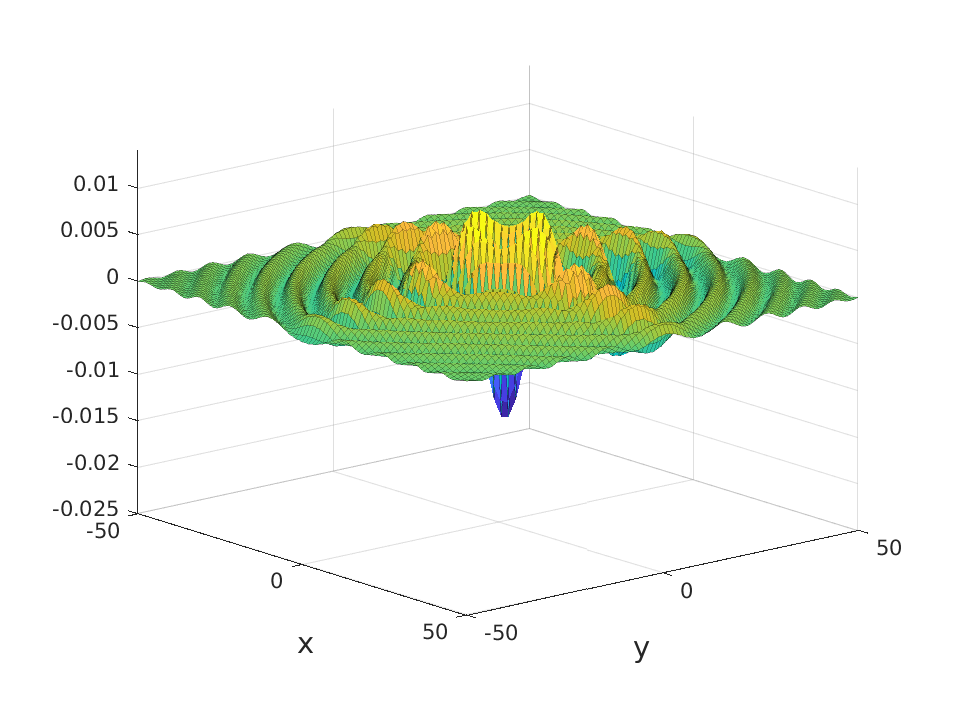
\includegraphics[scale=0.4]{conv}
	\includegraphics[scale=0.45]{conv-1}\\
	\includegraphics[scale=0.55]{conv-2}
	\includegraphics[scale=0.5]{conv-3}\\
	\includegraphics[scale=0.4]{conv-4}
	\includegraphics[scale=0.4]{conv-5}
\end{figure}








\newpage

\noindent \textbf{3.} I'm still running the calculations for $H^t_P(x,y)$ again with $t = 100$. The output looks good. I'm integrating in ``batches'' and will aggregate the data as I go along. This should give us a lot of data for future stretching/contracting/scaling at different values of $t$. Below is the first few batches (around the origin). The peaks have the correct orientation, and are very much like the convolution powers we've been generating!

\begin{figure}[!htb]
	\centering
	\includegraphics[scale=0.15]{conv-6}
	\includegraphics[scale=0.2]{conv-7}
	\includegraphics[scale=0.3]{conv-8}
\end{figure}


This is what I have as of March 9 and March 21, 2020:
\begin{figure}[!htb]
	\centering
	\includegraphics[scale=0.45]{conv-9}
	\includegraphics[scale=0.4]{conv-10}
\end{figure}



There are about $2\times 10^5$ data points in the second figure. 







\newpage

\noindent \textbf{4.} Here's the Python code I use to calculate the convolution powers
\begin{lstlisting}
import numpy as np
import matplotlib.pyplot as plt
from scipy import signal
from matplotlib import cm, colors
from mpl_toolkits.mplot3d.axes3d import Axes3D
import operator
import time
from numpy import unravel_index


def fast_convolve(n_times, support_bound, drift):
	Phi = np.zeros(shape=(9,9),dtype=np.complex_)

	Phi[ 0+9//2][ 0+9//2]  = complex(301/384,-7/48)
	Phi[ 0+9//2][-1+9//2]  = complex(7/96,1/24)     
	Phi[ 0+9//2][ 1+9//2]  = complex(3/32,1/24)      
	Phi[ 0+9//2][ 2+9//2]  = -1/48               
	Phi[ 0+9//2][-2+9//2]  = -1/48
	Phi[ 1+9//2][ 0+9//2]  = complex(7/96,1/24)
	Phi[-1+9//2][ 0+9//2]  = complex(7/96,1/24)
	Phi[ 2+9//2][ 0+9//2]  = -complex(7/192,1/96)
	Phi[-2+9//2][ 0+9//2]  = -complex(7/192,1/96)
	Phi[ 3+9//2][ 0+9//2]  = 1/96
	Phi[-3+9//2][ 0+9//2]  = 1/96
	Phi[ 4+9//2][ 0+9//2]  = -1/768
	Phi[-4+9//2][ 0+9//2]  = -1/768
	Phi[-1+9//2][-1+9//2]  =  1/192
	Phi[ 1+9//2][-1+9//2]  =  1/192
	Phi[ 1+9//2][ 1+9//2]  = -1/192
	Phi[-1+9//2][ 1+9//2]  = -1/192

	conv_power = np.copy(Phi)
	offset = np.array([0,0])

	i=0
	if drift:
		while i < n_times:
			i += 1
			init_vec = unravel_index(np.absolute(conv_power).argmax(), np.absolute(conv_power).shape)
			conv_power = signal.convolve2d(Phi, conv_power, 'full')
			after_vec = unravel_index(np.absolute(conv_power).argmax(), np.absolute(conv_power).shape)
			offset += np.subtract(init_vec , after_vec)

			dim_f = np.shape(conv_power)
	
			if dim_f[0] > support_bound or dim_f[0] > support_bound:
				conv_power = crop(conv_power, support_bound)
	else:
		while i < n_times:
			i += 1
			conv_power = signal.convolve2d(Phi, conv_power, 'full')
			dim_f = np.shape(conv_power)

			if dim_f[0] > support_bound or dim_f[0] > support_bound:
				conv_power = cropND(conv_power, support_bound)
return conv_power

def cropND(img, sup_bd):
	if sup_bd < np.shape(img)[0] and sup_bd < np.shape(img)[1]:
	dim = np.shape(img)
	return img[(dim[0]//2)-sup_bd//2:(dim[0]//2)+sup_bd//2,
		(dim[1]//2)-sup_bd//2:(dim[1]//2)+sup_bd//2]

def crop(img, sup_bd):
	center = unravel_index(np.absolute(img).argmax(), np.absolute(img).shape)
	return img[center[0]-sup_bd//2:center[0]+sup_bd//2,
		center[1]-sup_bd//2:center[1]+sup_bd//2]

if __name__ == '__main__':

while True:

	n_times = int(input('Convolve how many times? '))
	support_bound = int(input('NxN suppport bound, N = '))
	drift_ans = str(input('Expect asymetric drift? [y/n]: '))
	print('Calculating...')
	start = time.time()

	if drift_ans == 'y':
		drift = True
	elif drift_ans == 'n':
		drift = False
	else:
		print('WARNING: Write "y" for YES and "n" for NO.')
		print('------------------------------------------')
		print('\n')
		continue

	data = np.real(fast_convolve(n_times, support_bound, drift))
	dim = np.shape(data)
	x = range((-dim[0]//2)+1,(dim[0]//2)+1)
	y = range((-dim[1]//2)+1,(dim[1]//2)+1)

	hf = plt.figure()
	ha = hf.add_subplot(projection='3d')
	ha.set_xlim(-np.shape(data)[0]//2, np.shape(data)[0]//2)
	ha.set_ylim(-np.shape(data)[0]//2, np.shape(data)[0]//2)

	drift = False # I'm setting this for now for testing
	if drift:
		ha.set_xlabel('\n \n X \n \n DRIFTING CONVOLUTION POWERS!')
		ha.set_ylabel('\n \n Y \n \n DRIFTING CONVOLUTION POWERS!')
		ha.set_zlabel(' \n \n Re(Phi^(n)) for n='+str(n_times))
	else:
		ha.set_xlabel('X')
		ha.set_ylabel('Y')
		ha.set_zlabel(' \n \n Re(Phi^(n)) for n='+str(n_times))

	X, Y = np.meshgrid(x, y)  
	surf = ha.plot_surface(X, Y, data , rstride=1, cstride=1, cmap='plasma', edgecolor='none', linewidth=0.2)

	end = time.time()
	print('Time elapsed (s): ', end - start)

	plt.show()
	print('-------------------------------------')
\end{lstlisting}



\newpage



\noindent \textbf{5.} Here's the Mathematica code that I use to approximate and plot the attractor:
\begin{lstlisting}
H[i_, j_] := NIntegrate[Cos[(-i*x/(100^(1/2)) - j*y/(100^(1/4)) - y^4/96 + y^2*x/96 - x^2/24)],
 {x, -11, 11}, {y, -11, 11}, PrecisionGoal -> 4, 
Method -> "OscillatorySelection"]
data = Flatten[
Table[{i, j, H[i, j]}, {i, -7, 7, 0.1}, {j, 7, 10, 0.1}], 1];
Export["ConvolutionPowers/data5.csv", data, "CSV"]


ListPlot3D[Import["ConvolutionPowers/data5.csv"], ColorFunction -> Hue, PlotRange -> Full]
\end{lstlisting}

The output looks something like 
\begin{figure}[!htb]
	\centering
	\includegraphics[scale=0.3]{conv-6}
\end{figure}



































	
\end{document}